\chapter{Implementation}
\label{Implementation}

Both Feeder and Explorer are implemented in Typescript, and they are using js-ipfs\footnote{\url{https://github.com/ipfs/js-ipfs}} implementation of IPFS node. This environment selection allows code sharing between these two separated applications.

\section{Feeder implementation}
Informations about supported cryptocurrencies and enabled indexes are stored in Fedder's config file. Based on these settings, Feeder after start will begin to downloading data from Blockbook API, save them to IPFS, and create indexes of it.

\subsection{Indexes}
In the prototype, there are implemented a few different ways of indexing data in IPFS.
\begin{itemize}
    \item \textbf{OrbitDB}\footnote{\url{https://orbitdb.org/}} is a serverless, distributed, peer-to-peer database build on top of IPFS, developed by HAJA networks\footnote{\url{https://haja.io/}}. OrbitDB is a good solution for small user's databases, but it is still in the alpha stage of developing, and it is not well optimized to store hundreds of gigabytes of data. The biggest problem is that OrbitDB performs all queries locally. To perform query like \texttt{db.query((tx) => tx.amount > 0.001)} OrbitDB needs to load all database locally and then cycling between them. So every client ends up with a full copy of the database. This limitation is not usable for our case when we have a database that has hundreds of gigabytes of data.
    \cite{OrbitDBManual}
    \item \textbf{Textile}\footnote{\url{https://textile.io/}} is a set of open-source tools that provide a decentralized database, remote storage, user management, and more, over the IPFS network. Textile already created applications for storing photos\footnote{\url{https://textile.photos/}}, notes\footnote{\url{https://noet.io/}} or anything else\footnote{\url{https://anytype.io/}}. Textile provides a high abstraction on top of the IPFS and provides simple API to store and index files securely. It uses \textit{Cafe} peers to provides backups and indexing. Every data store is duplicated on several \textit{Cafe} peers. When a client is obtaining some data, it will contact one of the \textit{Cafe} peers, and \textit{Cafe} peer will resolve a query for the client. This is a problem for our solution because using textile require lots of harddisk memory and does not solve the problem with overloading \textit{Cafe} peers.
    \cite{TextileWhitePaper}
\end{itemize}

After some research, I came to the conclusion that currently, there is no solution for storing and indexing data in IPFS without high harddisk memory consummation. So I created my own indexing system that currently supports three types of indexes.

\begin{itemize}
    \item \textbf{Dictionary} - a simple key-value structure that can be used for translating (for example, block height to block). Search complexity is \texttt{O(1)}, which is the fastest achievable speed. Big disadvantage is that client needs to download a whole dictionary to performs search. In the time of writing this thesis, Ethereum has 9 250 000 blocks. If we want to make dictionary for translating block height to IPFS block address, the size of this dictionary would be at least \texttt{(int\_size + multihash\_size) * 9 250 000 } where minimal size for \texttt{int\_size} is \texttt{4} bytes and \texttt{multihash\_size} is \texttt{36} bytes when sha-256 is used (32 bytes) and multihash prefix is 4 bytes long. So this dictionary would have over 1.3 GB only for Ethereum. Another disadvantage is the impossibility to performing range search (for example get blocks between 9 249 950 and 9 250 000).

    \begin{figure}[h]
        \centering
        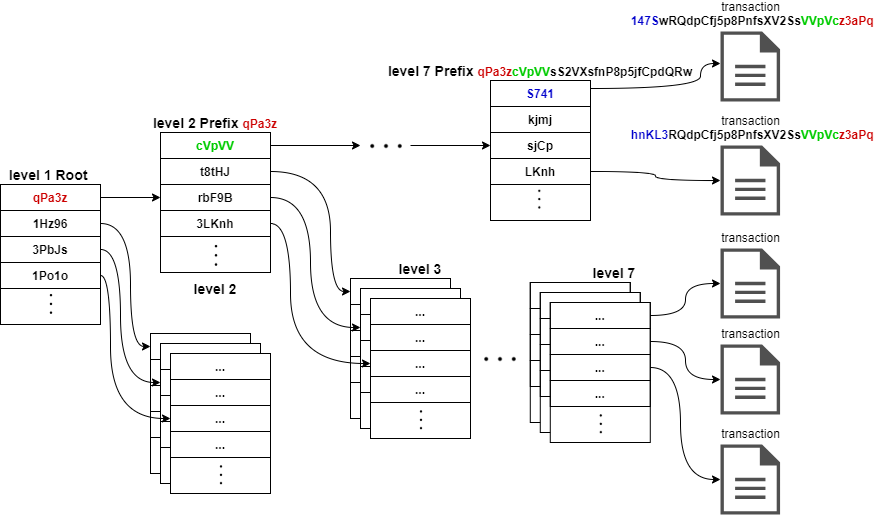
\includegraphics[width=13cm]{ReverseLookup_index.png}
        \caption{Reverse lookup by transaction hash}
        \label{reverseLookupIndex}
    \end{figure}


    \item \textbf{Reverse lookup} - this structure is inspired by Reverse DNS lookup\footnote{\url{https://en.wikipedia.org/wiki/Reverse_DNS_lookup}} and it's principle can be seen on figure \ref{reverseLookupIndex}. For every item that will be stored in this index, the key is reversed (for better selectivity) and split into the smaller substrings. Leading substring of every key is stored in root (level 1) dictionary and is pointing to another dictionary that consists of following substrings which have the corresponding prefix in parent dictionary. Last level dictionary substrings are pointing to IPFS objects. In this index, there is a problem with performing range select operations, because items have reversed key.
    \item \textbf{B+ Tree} - perhaps most powerfull index structure. With auto balanced B+ tree, we can efficiently search objects by given key and performs range selects. Example of this structure can be seen in figure \ref{btreeindex}. By default, there is the limit of 32 items in one node (but can be changed from 4 to 256). 
    


    \begin{figure}[h]
        \centering
        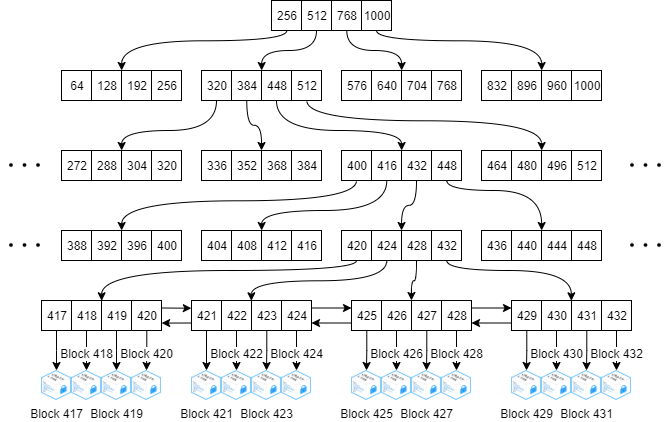
\includegraphics[width=13cm]{btreeindex.png}
        \caption{B+ tree index structure}
        \label{btreeindex}
    \end{figure}

\end{itemize}

Implementing these indexes in IPFS was surprisingly simple thanks to IPLD objects and links.


\section{Explorer implementation}
Currently, there are two options for running Explorer. First one is running Explorer like web application in a browser and the second one is to use Explorer as RestAPI. This architecture is shown in figure \ref{ExplorerArchitecture}.

\begin{figure}[h]
    \centering
    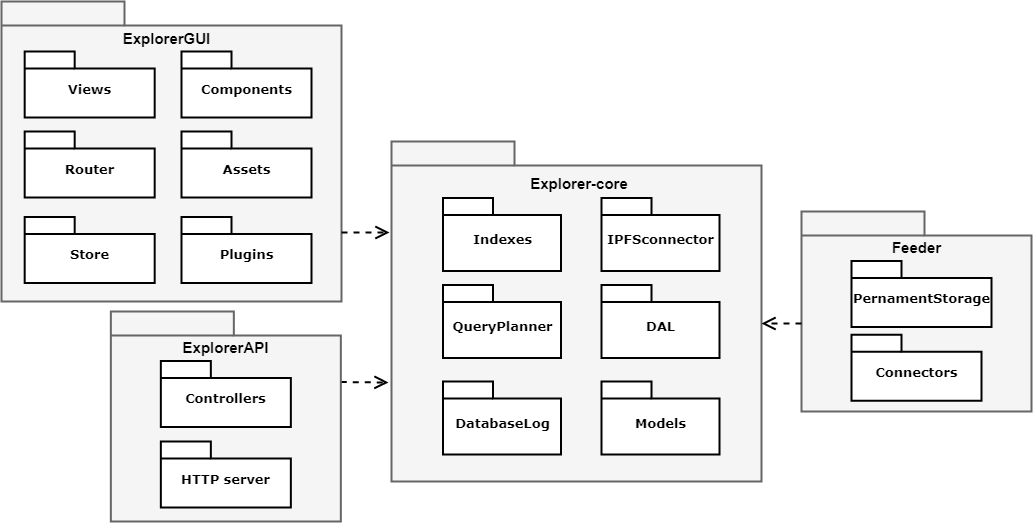
\includegraphics[width=13cm]{ExplorerArchitecture.png}
    \caption{Explorer architecture}
    \label{ExplorerArchitecture}
\end{figure}

\subsection{ExplorerCore}
ExplorerCore is module that communicate with IPFS. It has simple interface for obtaining the data:
\begin{itemize}
    \item \texttt{getTx(txHash)} - get transaction by its hash,
    \item \texttt{getBlock(blockHash)} - get block by its hash,
    \item \texttt{getBlock(blockHeight)} - get block by its height,
    \item \texttt{getAddress(addressHash)} - get address by its hash,
    \item \texttt{useIndex(index\_name, filter)} - use index to retrieve array of objects that fits \texttt{filter}.
\end{itemize}

\subsection{ExplorerGUI}
Running in browser with GUI module provides simple user interface implemented as a single page application. Browser's implementation of IndexedDB is used as a storage for IPFS as can be seen in figure \ref{browserIPFS}. Communication with other peers is provided though WebRTC\footnote{\url{https://webrtc.org/}} or WebSockets. Every tab opened in the browser is the same IPFS node. Opening a new tab in Incognito mode or different browser will spawn different IPFS node.

\begin{figure}[h]
    \centering
    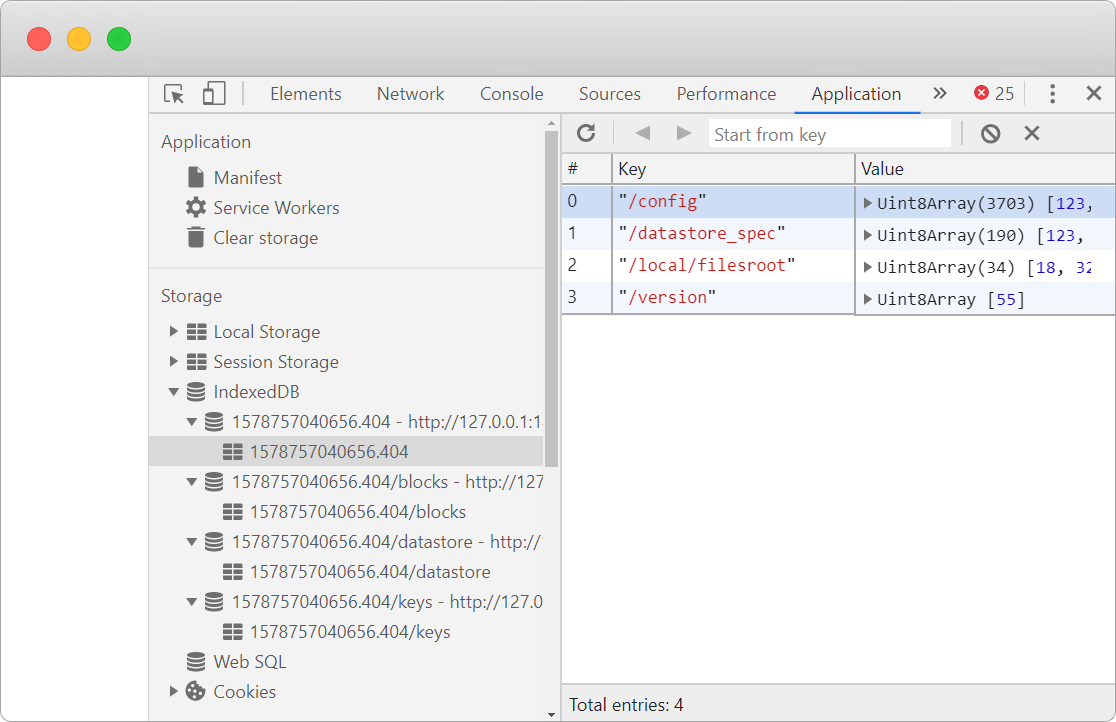
\includegraphics[width=12cm]{ipfsBrowser.PNG}
    \caption{IPFS storage in browser}
    \label{browserIPFS}
\end{figure}


\subsection{ExplorerAPI}
Node.js\footnote{\url{https://nodejs.org/}} implementation of IPFS uses filesystem to store data (figure \ref{nodeIPFS}). On the top of ExplorerCore, there is a simple web framework Express\footnote{\url{http://expressjs.com/}}, where are routes (endpoints) defined. Currently supported routes are described in table \ref{tab:explorerApiEndpoints}. Every route supports query parameters \texttt{filter} uses for filtering results and \texttt{limit} which limits number of results. Pagination can be made by setting \texttt{filter} to be greater/smaller (depending on ordering) as key of the last displayed object and \texttt{limit} to page size. For example, if a user is looking at page of transactions ordered by time (ordered from the newest transactions to the oldest), the next page of transactions are first \(N\) transactions that happened before last displayed transaction (where \(N\) is page size).

Rest API supports optional path param/s \texttt{path} that is useful for traversing objects in IPFS. If we want to get fifth transaction of the block with height 1000 one of the way is request URL \texttt{/block/998/next\_block/next\_block/txs/5} (get block with height 998, get next block two times, get transaction, a get fifth item from array of transactions). This approach allows the user to explore IPFS storage as graph very quickly by objects links.

\begin{figure}[h]
    \centering
    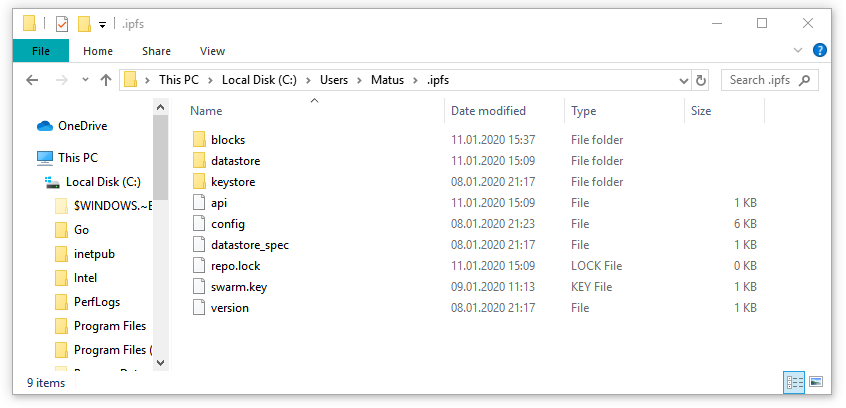
\includegraphics[width=12cm]{ipfsNode.PNG}
    \caption{IPFS storage in node.js}
    \label{nodeIPFS}
\end{figure}


\begin{table}[h]
    \centering
    \begin{tabular}{|l|l|}
    \hline
    Endpoint                           & Description                       \\ \hline
    \texttt{/tx/\{txHash\}/\{path*\}}           & Get transaction by hash  \\ \hline
    \texttt{/block/\{blockHeight\}/\{path*\}}   & Get block by height      \\ \hline
    \texttt{/block/\{blockHash\}/\{path*\}}     & Get block by hash        \\ \hline
    \texttt{/address/\{addressHash\}/\{path*\}} & Get address by hash      \\ \hline
    \end{tabular}
    \caption{Rest API explorer endpoints}
    \label{tab:explorerApiEndpoints}
\end{table}